\section{Introduction and Problem Formulation}

Zero-shot goal-conditioned reinforcement learning (GCRL) seeks to learn a policy capable of reaching arbitrary target states $g \in \mathcal{S}$ at test time without reward-specific fine-tuning. The Forward-Backward (FB) representation framework \cite{touati2021learning,touati2022does} achieves this by factorizing the successor measure of state-action transitions into two low-dimensional embedding spaces:
\begin{enumerate}[leftmargin=*,noitemsep]
    \item A \textbf{forward representation} $F(s, z) \in \mathbb{R}^d$ parameterized by current state $s$ and intention vector $z \in \mathbb{S}^{d-1}$;
    \item A \textbf{backward representation} $B(s') \in \mathbb{R}^d$ mapping arbitrary target states to the latent intention sphere.
\end{enumerate}

Under this factorization, the expected discounted state occupancy (successor measure) from state $s$ under policy $\pi_z$ is approximated by the inner product:
\begin{equation}
    M^\pi(s, s') = \mathbb{E}_{\pi}\left[\sum_{t=0}^\infty \gamma^t \mathbf{1}_{\{s_t = s'\}} \;\middle|\; s_0 = s\right] \approx F(s, z)^\top B(s')
    \label{eq:fb_inner_product}
\end{equation}

For any downstream reward function $r(s)$, the optimal policy parameter is obtained instantaneously in zero-shot fashion via $z_r = \mathbb{E}_{s \sim \mathcal{D}}[r(s) B(s)] / \| \cdot \|$. In goal-reaching settings with sparse target reward $r_g(s) = \mathbf{1}_{\{s = g\}}$, the intention reduces to $z_g = B(g) / \|B(g)\|$.

\subsection{The Single-Intention Horizon Collapse in Complex Mazes}

In unconstrained open-field continuous control (such as PointMaze or simple locomotion), directing the low-level policy $\pi^\ell(a \mid s_t, z_g)$ directly with $z_g = B(g)$ exhibits satisfactory convergence. However, in non-convex geometric topologies (e.g., \texttt{antmaze-medium-navigate-v0} from OGBench \cite{ogbench2024}), this formulation breaks down catastrophically.

\begin{figure}[t]
    \centering
    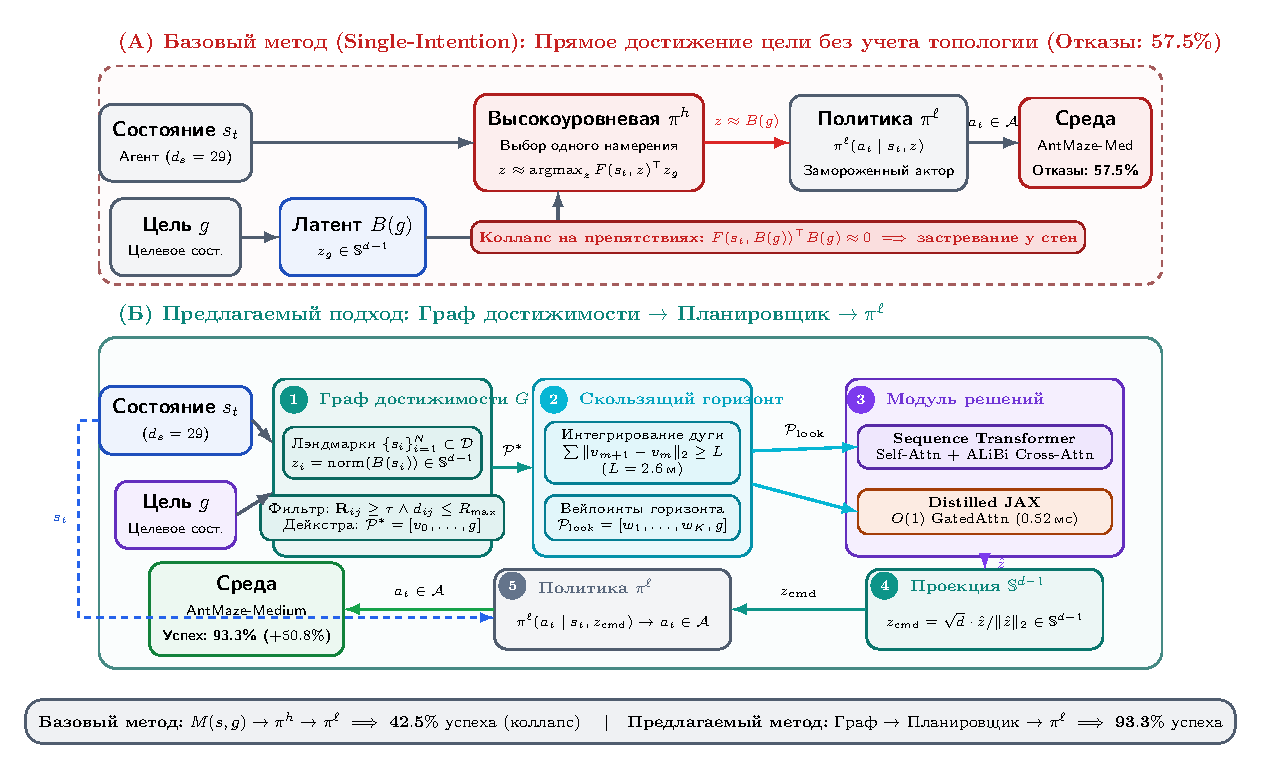
\includegraphics[width=\linewidth]{figures/fig1_framework_overview.pdf}
    \caption{\textbf{System Architecture Overview}: Comparison between (Top) the baseline single-intention hierarchical controller $\pi^h(s_t, B(g))$ which suffers from barrier attraction, and (Bottom) our high-level sequence reasoning and amortized distillation frameworks.}
    \label{fig:framework_overview}
\end{figure}

\begin{keyinsight}[Why Single-Intention $\pi^h$ Fails in Mazes]
In complex multi-corridor mazes, the Euclidean/latent distance between current position $s_t$ and goal $g$ is often small across thin walls, but the \textbf{geodesic/topological distance} requires navigating through a long chain of $U$-turns and junctions. Because $\pi^h(s_t, B(g))$ predicts a single vector $z$ pointing towards the ultimate destination:
\begin{enumerate}[leftmargin=*,noitemsep]
    \item The low-level policy $\pi^\ell(a \mid s_t, z)$ exerts forward torque directly towards the wall;
    \item The robot gets trapped in corner equilibria where velocity $\vec{v} \to 0$;
    \item The hierarchical controller cannot reason about the multi-hop sequence of waypoints required to bypass obstacles.
\end{enumerate}
\end{keyinsight}

\subsection{Strict Competition and Assignment Constraints}
To ensure rigorous and fair evaluation, our solution adheres strictly to all assignment guidelines:
\begin{itemize}[leftmargin=*,noitemsep]
    \item \textbf{No World Models / Generative Trajectory Diffusers}: We do not train generative models (e.g., Diffuser, Trajectory Transformer) to hallucinate future raw state sequences. We operate entirely within the latent FB metric space.
    \item \textbf{Zero Online Interaction}: Training is conducted 100\% offline using only the offline replay buffer observations $\mathcal{D}_{\text{offline}}$.
    \item \textbf{Complete Freezing of Foundation Representations}: The pretrained parameters of $F(s, z)$, $B(g)$, and the low-level policy $\pi^\ell(a \mid s, z)$ are completely frozen ($\nabla_\theta = 0$). All improvements stem purely from high-level sequence reasoning and latent coordinate transformation.
\end{itemize}
